\section{Experiments}\label{sec:experiment}
We experimentally evaluated the performance and quality of our methodology, and corresponding heuristic implementation in \cref{subsec:heuristics},
and compare them against the exhaustive approach in Section~\cref{TOADD}. In the following,
\cref{subsec:experiments_infrastructure} presents the simulator and testing infrastructure adopted in our experiments, as well as the complete experimental settings; \cref{subsec:experiments_performance} analyses the performance of our solution in terms of execution time; \cref{subsec:experiments_quality} presents the quality of our heuristic algorithm in terms of the metrics in \cref{subsec:metrics}.

\subsection{Testing Infrastructure and Experimental Settings}\label{subsec:experiments_infrastructure}
Our testing infrastructure is a Swift-based simulator of a service-based ecosystem, including service execution, comparison, and composition.
The simulator first defines the pipeline template as a sequence of vertexes in the range $3-7$.
We recall that alternative vertexes are modeled in different pipeline templates,
while parallel vertexes only add a fixed execution time that is negligible and do not affect the quality of our approach.
Each vertex is associated with a (set of) policy with transformations varying in two classes:
\begin{itemize*}
  \item \average: data removal percentage within $[0.5,0.8]$.
  \item \wide:    data removal percentage within $[0.20,1]$.
\end{itemize*}

Upon setting the sliding window size, the simulator selects a subset of vertexes along with their corresponding candidate services.
It then generates all possible service combinations for the chosen vertexes.
For each combination, the simulator calculates a metric and selects the first service from the optimal combination before shifting the sliding window.
When the end of the vertex list is reached, or when the window size equals the vertex count, the simulator computes the optimal service combination for the remaining vertexes.

An hash function is to simulate the natural interdependence between services.
This is particularly important when the removal of data by one service may impact another.
By assigning weights to the services using this function, the system aims to reflect the interconnected dynamics among the services.

The simulator is used to assess the performance and quality of our sliding window heuristic in Section \ref{sec:heuristics} for the generation of the best pipeline instance (Section \ref{sec:instance}).
% Performance measures the heuristics execution time in different settings, while quality compares the results provided by our heuristics in terms of selected services with the optimal solution retrieved using the exhaustive approach.
%We note that the exhaustive approach generates the best pipeline instance by executing all possible combinations of candidate services.
%The emulator simplifies the execution of the service composition by removing the service selection phase, which is not relevant for the purpose of the experiment.
Our experiments have been run on a workstation equipped with a 2.40GHz i5-8279U CPU with 16GB RAM and a 512GB SSD.
Each experiment was repeated ten times and the results averaged to improve the reliability of the data.



\begin{figure}[!t]
  \centering
  \resizebox{\columnwidth}{!}{%
    \begin{tikzpicture}[framed]
      \node[draw, circle,fill=red!20] (s41) at (1,1.7) {$\sii{1}$};
      \node[draw, circle, fill=green!20] (s42) at (1,0) {$\sii{2}$};
      \node[draw, circle, fill=red!20] (s43) at (1,-1.7) {$\sii{3}$};

      \node[draw, circle] (s1) at (3,1.7) {$\sii{11}$};
      \node[draw, circle] (s2) at (3,0) {$\sii{12}$};
      \node[draw, circle] (s3) at (3,-1.7) {$\sii{13}$};

      \node[draw, circle] (s11) at (5,1.7) {$\sii{21}$};
      \node[draw, circle] (s12) at (5,0) {$\sii{22}$};
      \node[draw, circle] (s13) at (5,-1.7) {$\sii{23}$};

      \node[draw, circle] (s21) at (7,1.7) {$\sii{31}$};
      \node[draw, circle] (s22) at (7,0) {$\sii{32}$};
      \node[draw, circle] (s23) at (7,-1.7) {$\sii{33}$};

      \node[draw, circle] (s31) at (9,1.7) {$\sii{41}$};
      \node[draw, circle] (s32) at (9,0) {$\sii{42}$};
      \node[draw, circle] (s33) at (9,-1.7) {$\sii{43}$};


      % \draw[->] (node2) -- (node3);
      \draw[->] (s42) -- (s1);
      \draw[->] (s42) -- (s2);
      \draw[->] (s42) -- (s3);

      \draw[->] (s1) -- (s11);
      \draw[->] (s1) -- (s12);
      \draw[->] (s1) -- (s13);

      \draw[->,dashdotted] (s2) -- (s11);
      \draw[->,dashdotted] (s2) -- (s12);
      \draw[->,dashdotted] (s2) -- (s13);

      \draw[->,dashed] (s3) -- (s11);
      \draw[->,dashed] (s3) -- (s12);
      \draw[->,dashed] (s3) -- (s13);


      \draw[->] (s11) -- (s21);
      \draw[->] (s11) -- (s22);
      \draw[->] (s11) -- (s23);

      \draw[->,dashdotted] (s12) -- (s21);
      \draw[->,dashdotted] (s12) -- (s22);
      \draw[->,dashdotted] (s12) -- (s23);

      \draw[->,dashed] (s13) -- (s21);
      \draw[->,dashed] (s13) -- (s22);
      \draw[->,dashed] (s13) -- (s23);


      \begin{scope}[on background layer]
        \draw[thick, dashed, fill=red!10, opacity=0.5]
        ([shift={(-0.5,0.5)}]s1.north west) rectangle ([shift={(0.5,-0.5)}]s23.south east);

      \end{scope}
    \end{tikzpicture}
  }
  \caption{Execution example}
  \label{fig:execution_example}
\end{figure}

\subsection{Perfomance}\label{subsec:experiments_performance}
% \subsection{performance}
% \begin{itemize}
%   \item Finestra scorrevole da 1 a N=Nodi
%   \item Servizi 5 a 20 passo 5 + 50??
%   \item
% \end{itemize}
% \subsection{Metriche/Euristiche}
We first calculated the execution time required by our exhaustive solution.
We incrementally varied the number of vertexes and the number of services per vertex.
The results of these evaluations are presented in \cref{fig:perf_exhaustive}.
As anticipated, the trend in execution times is exponential. \cref{fig:perf_exhaustive} displays the execution time plots,
clearly showing that as the number of vertexes increases, the execution time grows exponentially.
Execution times for up to 5 vertexes and 6 services were computed directly,
while the remaining data points were obtained through interpolation.
Subsequently, the logical extension of this empirical inquiry involves evaluating the execution time efficiency attributable to the implementation of the sliding window heuristic.

We then evaluated our heuristics to quantify the execution time reduction achieved through the application of heuristics.
In this context, the number of vertexes and services per vertex was incrementally increased,
with the addition of a sliding window whose size was progressively enlarged in each experiment.
The outcomes are depicted in \cref{fig:perf_window}, and as expected,
we observed a marked reduction in execution times with the implementation of the sliding window heuristic.
This empirical evidence highlights the heuristic's ability to reduce computational demands,
an aspect that becomes increasingly pivotal as the problem's complexity grows.
The use of a logarithmic scale to illustrate the results linearizes the exponential growth associated with the exhaustive method,
offering a clear visual confirmation of the heuristic's efficiency in decreasing computational time.
\begin{figure}[htb!]
  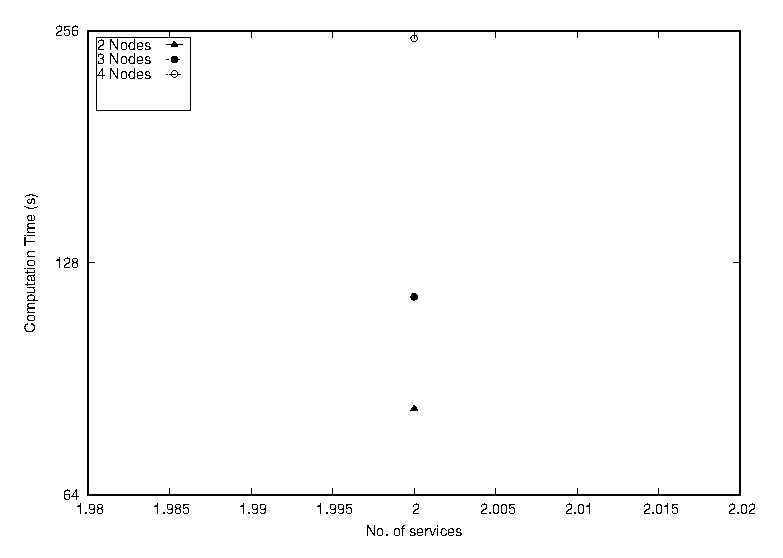
\includegraphics[width=0.95\columnwidth]{graphs/exhaustive_performance.eps}
  \caption{Exhaustive execution time evaluation. The x-axis represents the number of services, while the y-axis represents the execution time in seconds. The execution time is expressed both in linear and logarithmic scales.}
  \label{fig:perf_exhaustive}
\end{figure}


\subsection{Quality}\label{subsec:experiments_quality}
We finally evaluated the quality of our heuristic comparing, where possible, its results with the optimal solution retrieved by executing the exhaustive approach. The latter is executed with window size equals to the number of vertexes in the pipeline template, and provides the best, among all possible, solutions.

We run our experiments using the two settings in Section \cref{subsec:experiments_infrastructure}, namely, \average and \wide,  and varied: \emph{i)} the number of vertexes in the pipeline template in [3,7], \emph{ii)} the window size in [1,$|$max$_v$$|$], where max$_v$ is the number of vertexes in the pipeline template, and \emph{iii)} the number of candidate services for each vertex in the pipeline template in [2, 7].


\cref{fig:quality_window_average_perce,fig:quality_window_perce_wide} presents our results the quantitive metrics in \cref{subsec:metrics} for the \wide and \average settings, respectively.
Value are normalized to the optimal solution retrieved by the exhaustive approach.
%
When a \wide setting is employed, the average quality ratio in a configuration with three nodes for window of size one is 0.93, with a standard deviation of 0.02; it is 0.98 with a standard deviation of 0.01, when a window of size two is used. Increasing the number of nodes to four results in an average quality ratio of 0.88 for a window size of one with a standard deviation of 0.04, 0.96 with a standard deviation of 0.02,when a window of size two is used, 0.99 for a window size of three. Increasing to five nodes, the average quality ratio is 0.76 for a window size of one with a standard deviation of 0.09, 0.90 for a window of size two. Size two exhibited a standard deviation of 0.04, size three a standard deviation of 0.01, size 4 a standard deviation of 0.01.
For 6 nodes, the average quality ratio was 0.78 for a window of size one with a standard deviation of 0.09; 0.87 for a window of size two with a standard deviation of 0.04; 0.95 for a window of size three with a standard deviation of 0.02; 0.97 for a window of size four with a standard deviation of 0.02; and 0.99 for a window of size five.In a configuration of 7 nodes, the average quality ratio was 0.73 for a window sizeof one with a standard deviation of 0.08; it is 0.87 for a window size of size two, with a standard deviation of 0.08.  window size of 3 nodes exhibited a quality ratio of 0.95  with a standard deviation of 0.02, it is 0.96 for a window size of 4 nodes, with a standard deviation of 0.02. The mean value of the quality ratio is 0.99 for a window size of 5 and 6 nodes, with a standard deviation of 0.02.


When a \average setting is employed, in a configuration with three nodes and using a window size ranging from 1 to 2 the quality ratio is respectively: 0.95 and 0.99 with a standard deviation respectively of 0.017 and 0.006. For a configuration with four nodes and using a window size ranging from 1 to 3 the quality ratio is respectively: 0.93, 0.97 and 0.99 with a standard deviation respectively of 0.019, 0.006 and 0.007. For a configuration with five nodes and using a window size ranging from 1 to 4 the quality ratio is respectively:
0.88, 0.93, 0.97 and 0.98 with a standard deviation respectively of 0.02, 0.03, 0.015 and 0.016. For a configuration with six nodes and using a window size ranging from 1 to 5 the quality ratio is respectively:
0.87, 0.92, 0.96, 0.97 and 0.99 with a standard deviation respectively of 0.047, 0.058, 0.021, 0.014 and 0.004. For a configuration with seven nodes and using a window size ranging from 1 to 6 the quality ratio is respectively:
0.83, 0.92, 0.98, 0.98, 0.99 and 0.99 with a standard deviation respectively of 0.068, 0.030, 0.007, 0.017, 0.006 and 0.004.


\cref{fig:quality_window_wide_qualitative,fig:quality_window_average_qualitative} presents our results the qualitative metric in \cref{subsec:metrics} for the \wide and \average settings, respectively.
Value are normalized to the optimal solution retrieved by the exhaustive approach.

When a \wide setting is employed, in a configuration with three nodes and using a window size ranging from 1 to 2 the quality ratio is respectively: 0.98 and 0.998 with a standard deviation respectively of 0.014 and 0.005. For a configuration with four nodes and using a window size ranging from 1 to 3 the quality ratio is respectively: 0.97, 0.99, and 0.996 with a standard deviation respectively of 0.019, 0.004, and 0.004. For a configuration with five nodes and using a window size ranging from 1 to 4 the quality ratio is respectively:
0.93, 0.97, 0.993, and 0.998 with a standard deviation respectively of 0.022, 0.015, 0.006, and 0.003. For a configuration with six nodes and using a window size ranging from 1 to 5 the quality ratio is respectively:
0.92, 0.97, 0.995, 0.996, and 0.998 with a standard deviation respectively of 0.028, 0.018, 0.004, 0.005, and 0.003. For a configuration with seven nodes and using a window size ranging from 1 to 6 the quality ratio is respectively:
0.90, 0.96, 0.97, 0.994, 0.997, and 0.999 with a standard deviation respectively of 0.016, 0.019, 0.010, 0.005, 0.003, and 0.003.


When \average setting is employed, in a configuration with three nodes and using a window size ranging from 1 to 2 the quality ratio is respectively: 0.99 and 1.00 with a standard deviation respectively of 0.003, and 0.000.
For a configuration with four nodes and using a window size ranging from 1 to 3 the quality ratio is respectively:
0.98, 0.99, and 1.00 with a standard deviation respectively of 0.010, 0.003 and 0.003. For a configuration with five nodes and using a window size ranging from 1 to 4 the quality ratio is respectively:
0.98, 0.99, 1.00 and 1.00 with a standard deviation respectively of 0.004, 0.003, 0.004, and 0.000. For a configuration with six nodes and using a window size ranging from 1 to 5 the quality ratio is respectively:
0.97, 0.98, 1.00, 1.00 and 1.00 with a standard deviation respectively of 0.006, 0.003, 0.000, 0.003 and 0.003. For a configuration with seven nodes and using a window size ranging from 1 to 6  the quality ratio is respectively:
0.96, 0.98, 0.99, 0.99, 1.00 and 1.00 with a standard deviation respectively of 0.019, 0.009, 0.005, 0.005, 0.003 and 0.000.


% We note that the benefit of an increasing window size can be appreciated with lower numbers, reaching a sort of saturation around the average length (e.g., window of length 6 with a 7-vertex pipeline) where the quality ratio overlaps. The only exception is for 6-vertex pipeline where the overapping starts with window size 2. However, this might be due to the specific setting and therefore does not generalize.
% %Thus because the heuristic has more services to choose from and can find a better combination.
% We also observe that, as the window size increase, the quality increase as well. This suggests that the heuristic performs better when it has a broader perspective of the data it is governing.
% It's worth noting that lower window sizes are more unstable, with the quality ratio varying significantly between different configuration while higher window sizes tend to stabilize the quality ratio across different configuration.


\hl{QUESTO E' PIU' DA CONCLUSIONE FINALE.} Finally, the data suggest that while larger window sizes generally lead to better performance, there might exist a point where the balance between window size and performance is optimized. Beyond this point, the incremental gains in metric values may not justify the additional computational resources or the complexity introduced by larger windows.


\begin{figure*}[!htb]
  \centering
  \begin{subfigure}{0.33\textwidth}
    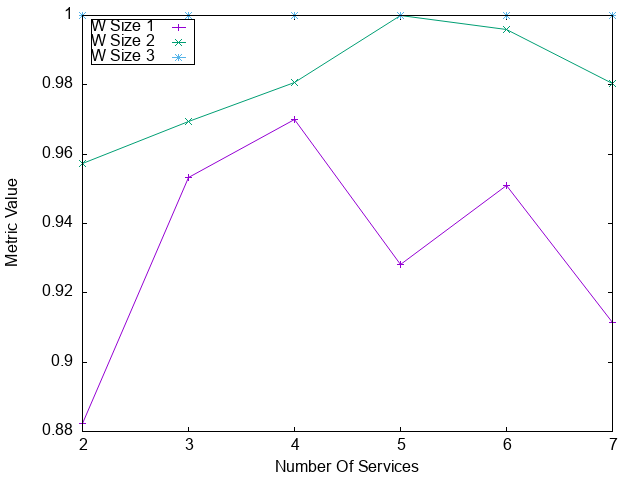
\includegraphics[width=\textwidth]{Images/graphs/newwindow_quality_performance_diff_perce_n7_s7_20_100_n3.png}
    \caption{3 vertices}
    \label{fig:quality_window_perce_wide_3n}
  \end{subfigure}
  \hfill
  \begin{subfigure}{0.33\textwidth}
    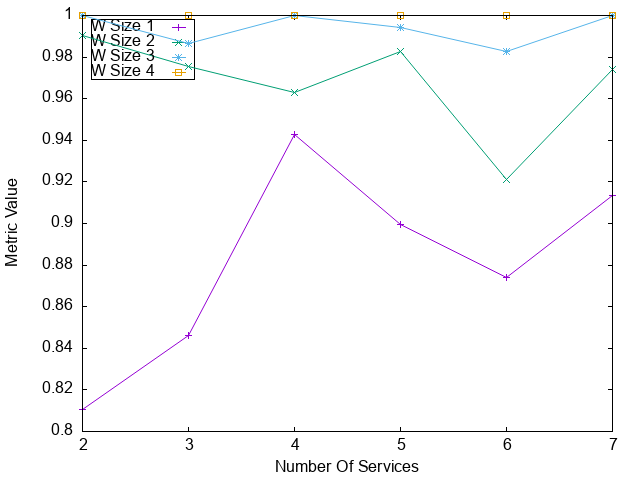
\includegraphics[width=\textwidth]{Images/graphs/newwindow_quality_performance_diff_perce_n7_s7_20_100_n4}
    \caption{4 vertices}
    \label{fig:quality_window_perce_wide_4n}
  \end{subfigure}
  \hfill
  \begin{subfigure}{0.33\textwidth}
    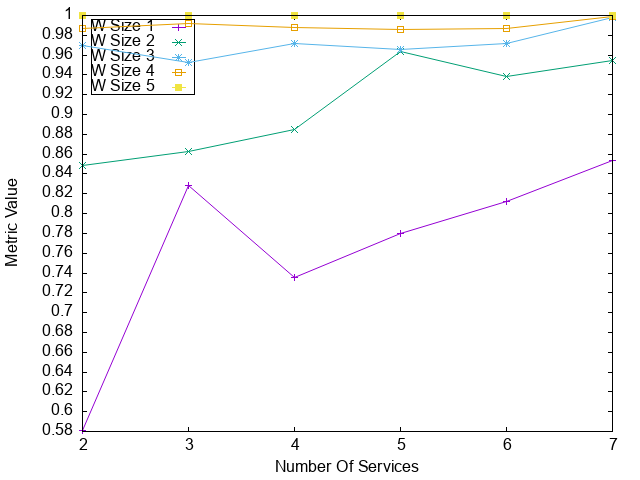
\includegraphics[width=\textwidth]{Images/graphs/newwindow_quality_performance_diff_perce_n7_s7_20_100_n5}
    \caption{5 vertices}
    \label{fig:quality_window_perce_wide_5n}
  \end{subfigure}
  \hfill
  \begin{subfigure}{0.33\textwidth}
    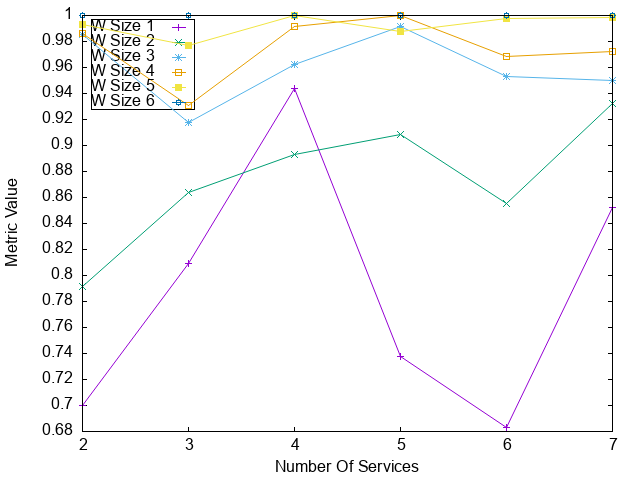
\includegraphics[width=\textwidth]{Images/graphs/newwindow_quality_performance_diff_perce_n7_s7_20_100_n6}
    \caption{6 vertices}
    \label{fig:quality_window_perce_wide_6n}
  \end{subfigure}
  \begin{subfigure}{0.33\textwidth}
    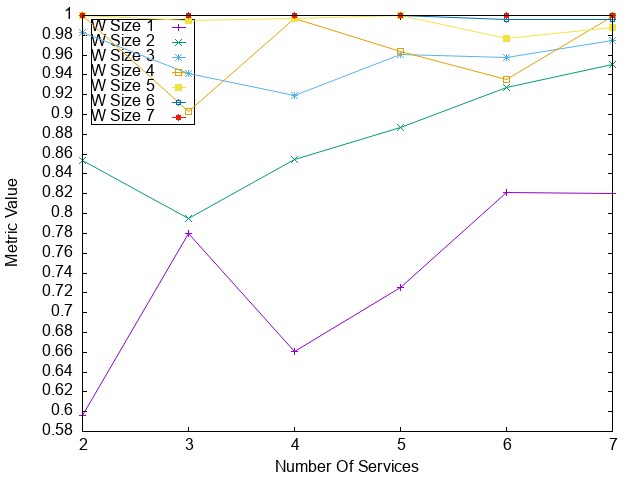
\includegraphics[width=\textwidth]{Images/graphs/newwindow_quality_performance_diff_perce_n7_s7_20_100_n7}
    \caption{7 vertices}
    \label{fig:quality_window_perce_wide_7n}
  \end{subfigure}
  % \hfill
  % \begin{subfigure}{0.33\textwidth}
  %   \includegraphics[width=\textwidth]{Images/graphs/quality_plot_average_n7.eps}
  %   \caption{7 vertices}
  %   \label{fig:third}
  % \end{subfigure}
  \caption{ Quality evaluation with \wide profile.}
  \label{fig:quality_window_perce_wide}
\end{figure*}


\begin{figure*}[!htb]
  \centering
  \begin{subfigure}{0.33\textwidth}
    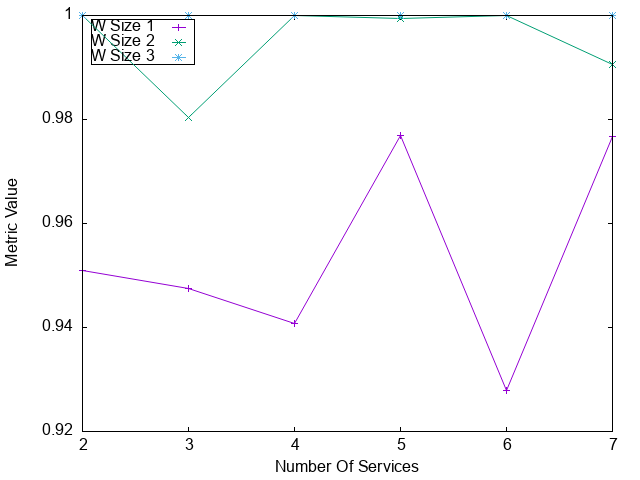
\includegraphics[width=\textwidth]{Images/graphs/newwindow_quality_performance_diff_perce_n7_s7_50_89_n3}
    \caption{3 vertices}
    \label{fig:quality_window_average_perce_3n}
  \end{subfigure}
  \hfill
  \begin{subfigure}{0.33\textwidth}
    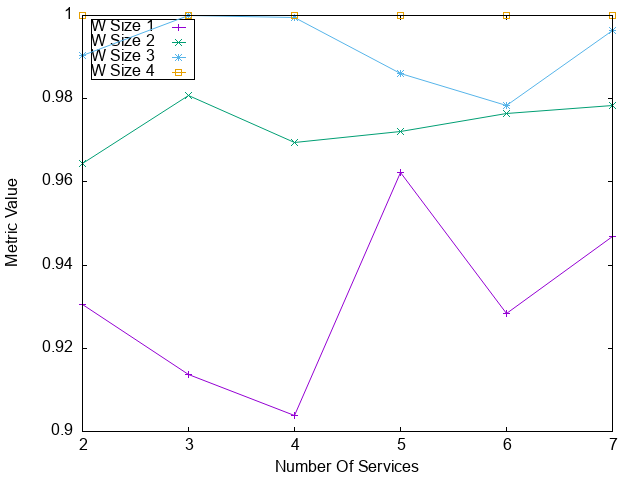
\includegraphics[width=\textwidth]{Images/graphs/newwindow_quality_performance_diff_perce_n7_s7_50_89_n4}
    \caption{4 vertices}
    \label{fig:quality_window_average_perce_4n}
  \end{subfigure}
  \hfill
  \begin{subfigure}{0.33\textwidth}
    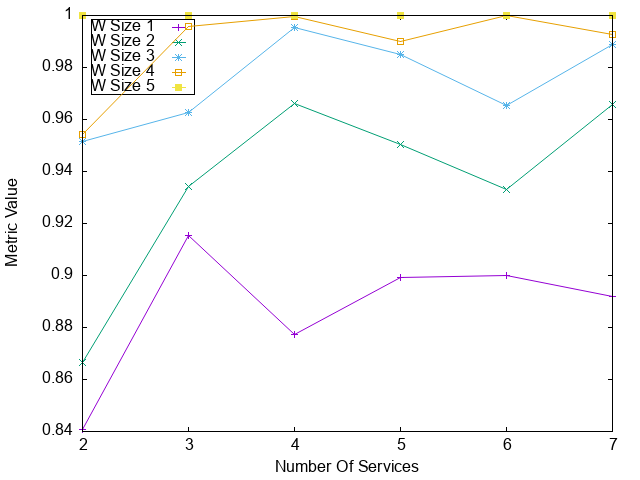
\includegraphics[width=\textwidth]{Images/graphs/newwindow_quality_performance_diff_perce_n7_s7_50_89_n5}
    \caption{5 vertices}
    \label{fig:quality_window_average_perce_5n}
  \end{subfigure}
  \hfill
  \begin{subfigure}{0.33\textwidth}
    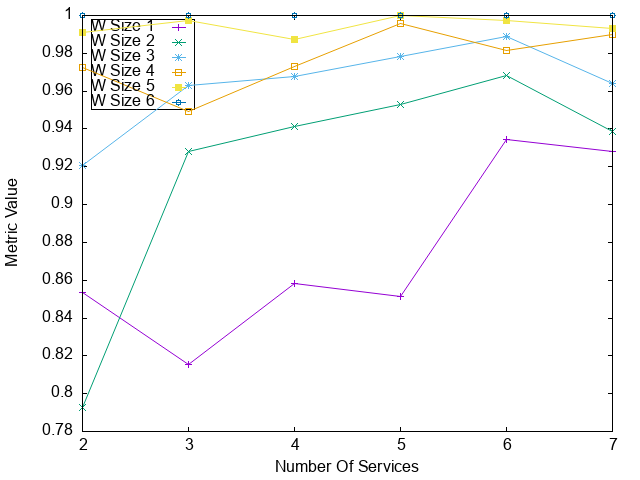
\includegraphics[width=\textwidth]{Images/graphs/newwindow_quality_performance_diff_perce_n7_s7_50_89_n6}
    \caption{6 vertices}
    \label{fig:quality_window_average_perce_6n}
  \end{subfigure}
  \begin{subfigure}{0.33\textwidth}
    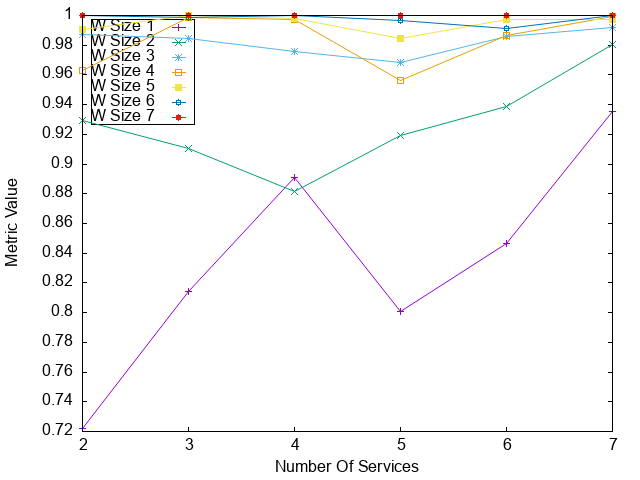
\includegraphics[width=\textwidth]{Images/graphs/newwindow_quality_performance_diff_perce_n7_s7_50_89_n7}
    \caption{7 vertices}
    \label{fig:quality_window_average_perce_7n}
  \end{subfigure}
  % \hfill
  % \begin{subfigure}{0.33\textwidth}
  %   \includegraphics[width=\textwidth]{Images/graphs/quality_plot_average_n7.eps}
  %   \caption{7 vertices}
  %   \label{fig:third}
  % \end{subfigure}
  \caption{ Quality evaluation with \average profile.}
  \label{fig:quality_window_average_perce}
\end{figure*}


\begin{figure*}[!htb]
  \centering
  \begin{subfigure}{0.33\textwidth}
    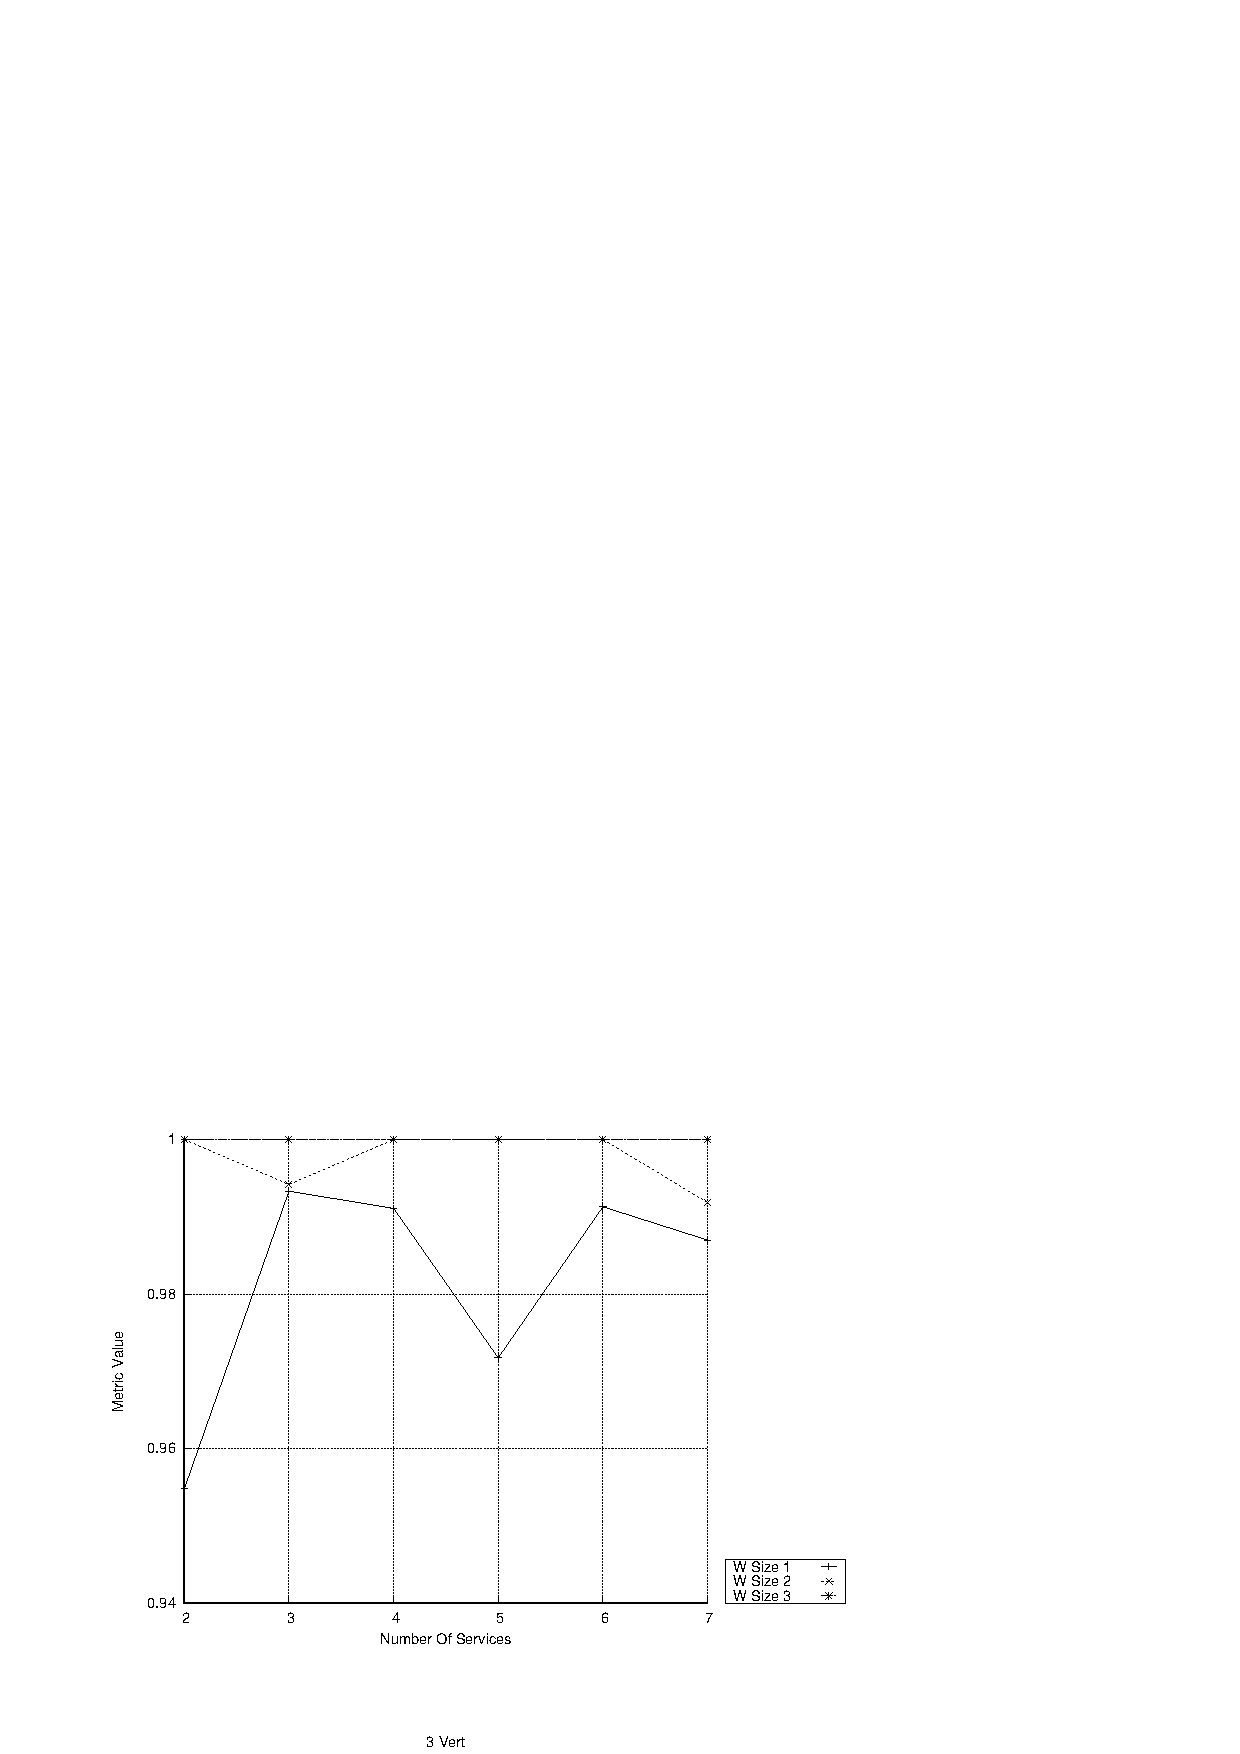
\includegraphics[width=\textwidth]{Images/graphs/window_quality_performance_diff_qual_n7_s7_20_100_n3}
    \caption{3 vertices}
    \label{fig:quality_window_wide_qualitative_n3}
  \end{subfigure}
  \hfill
  \begin{subfigure}{0.33\textwidth}
    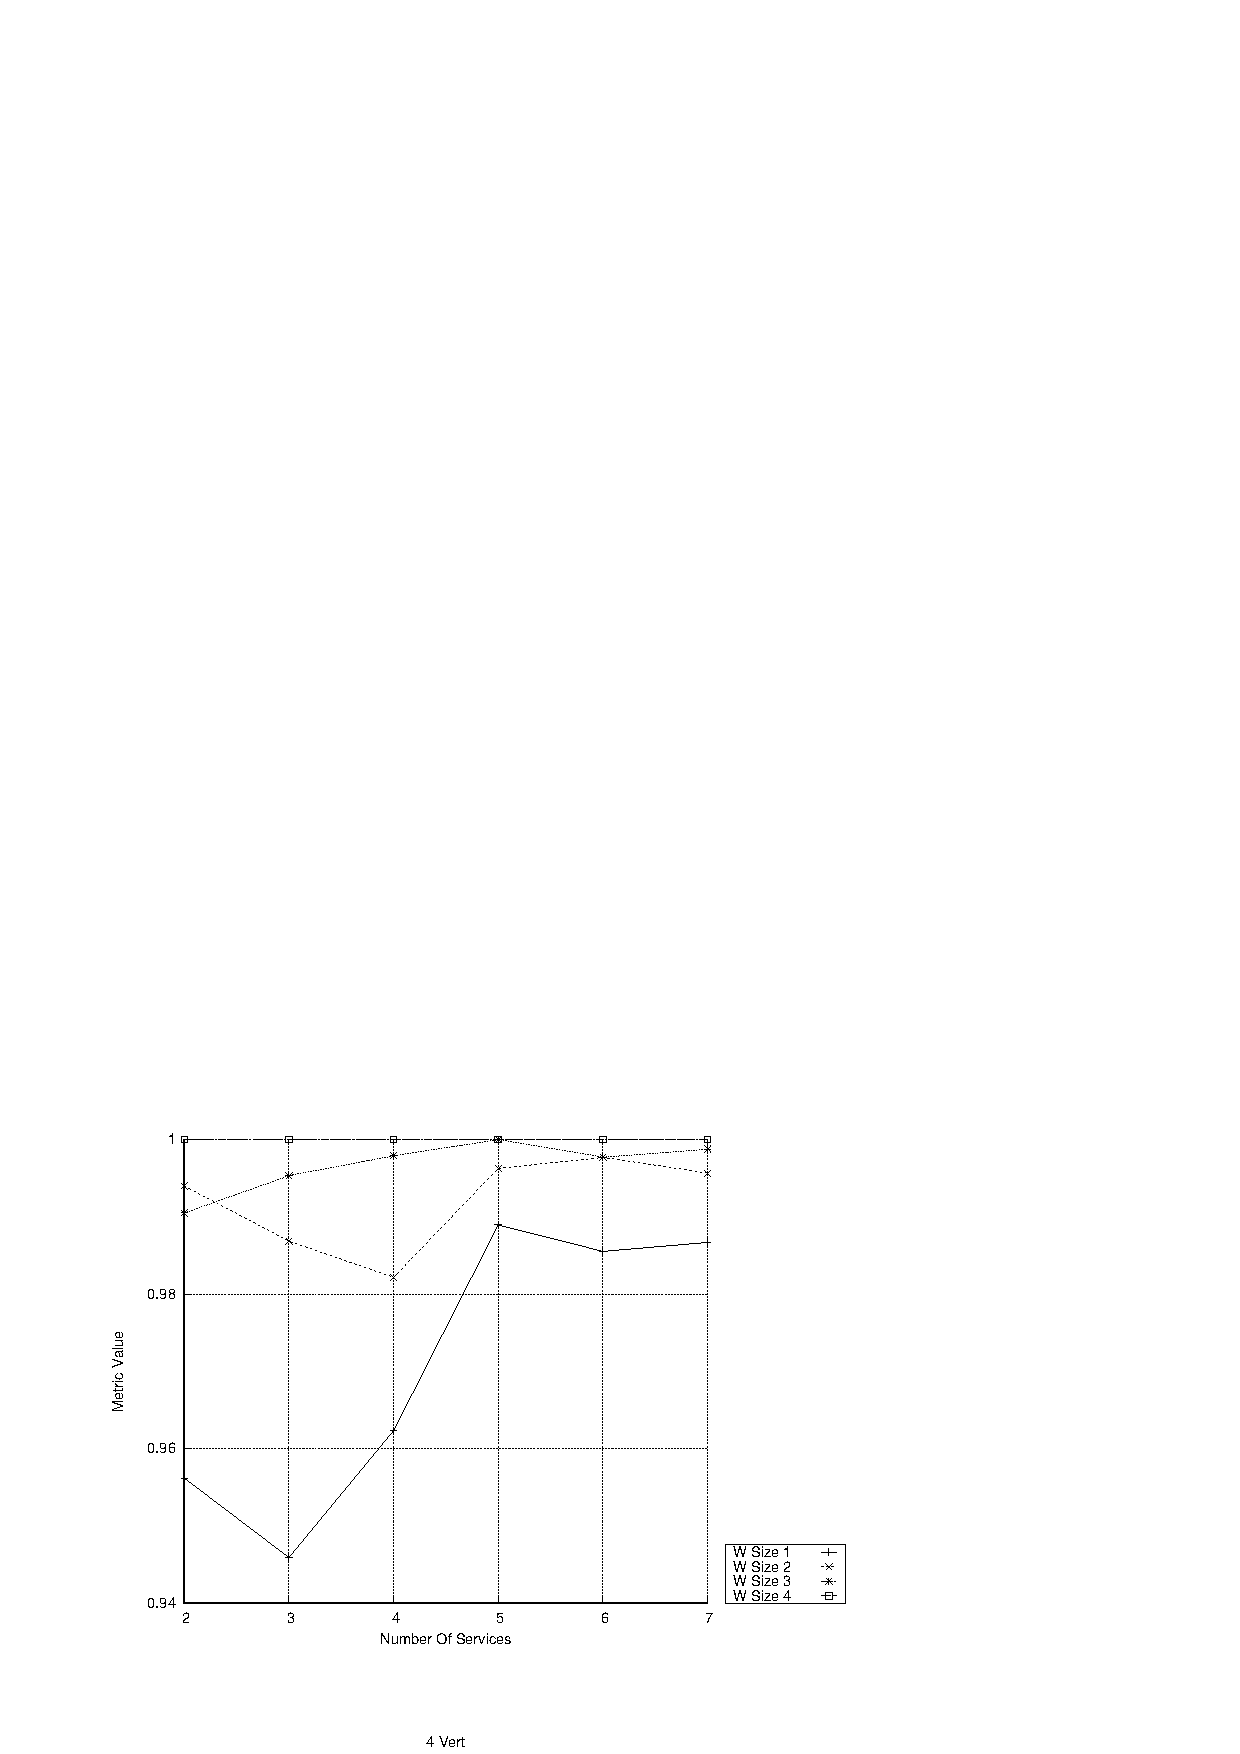
\includegraphics[width=\textwidth]{Images/graphs/window_quality_performance_diff_qual_n7_s7_20_100_n4}
    \caption{4 vertices}
    \label{fig:quality_window_wide_qualitative_n4}
  \end{subfigure}
  \hfill
  \begin{subfigure}{0.33\textwidth}
    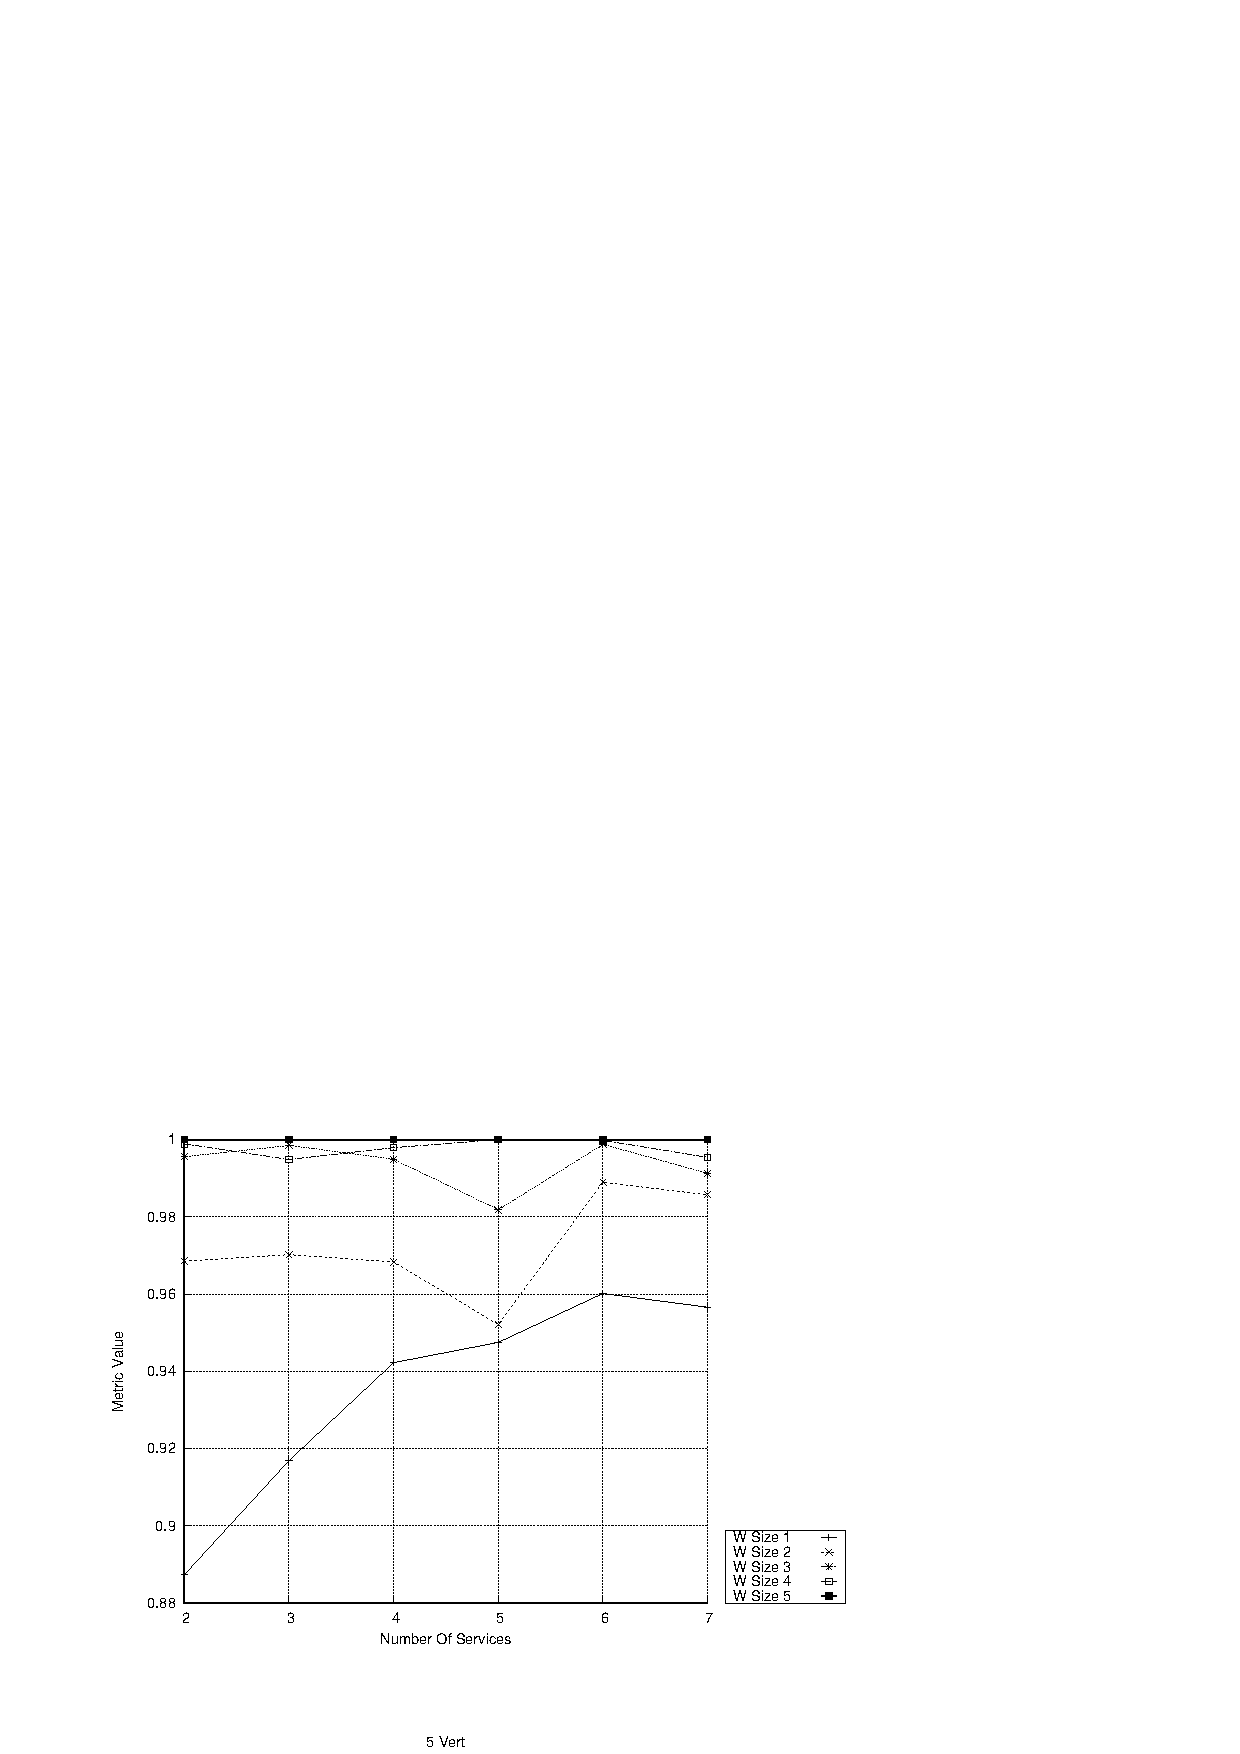
\includegraphics[width=\textwidth]{Images/graphs/window_quality_performance_diff_qual_n7_s7_20_100_n5}
    \caption{5 vertices}
    \label{fig:quality_window_average_qualitative_n5}
  \end{subfigure}
  \hfill
  \begin{subfigure}{0.33\textwidth}
    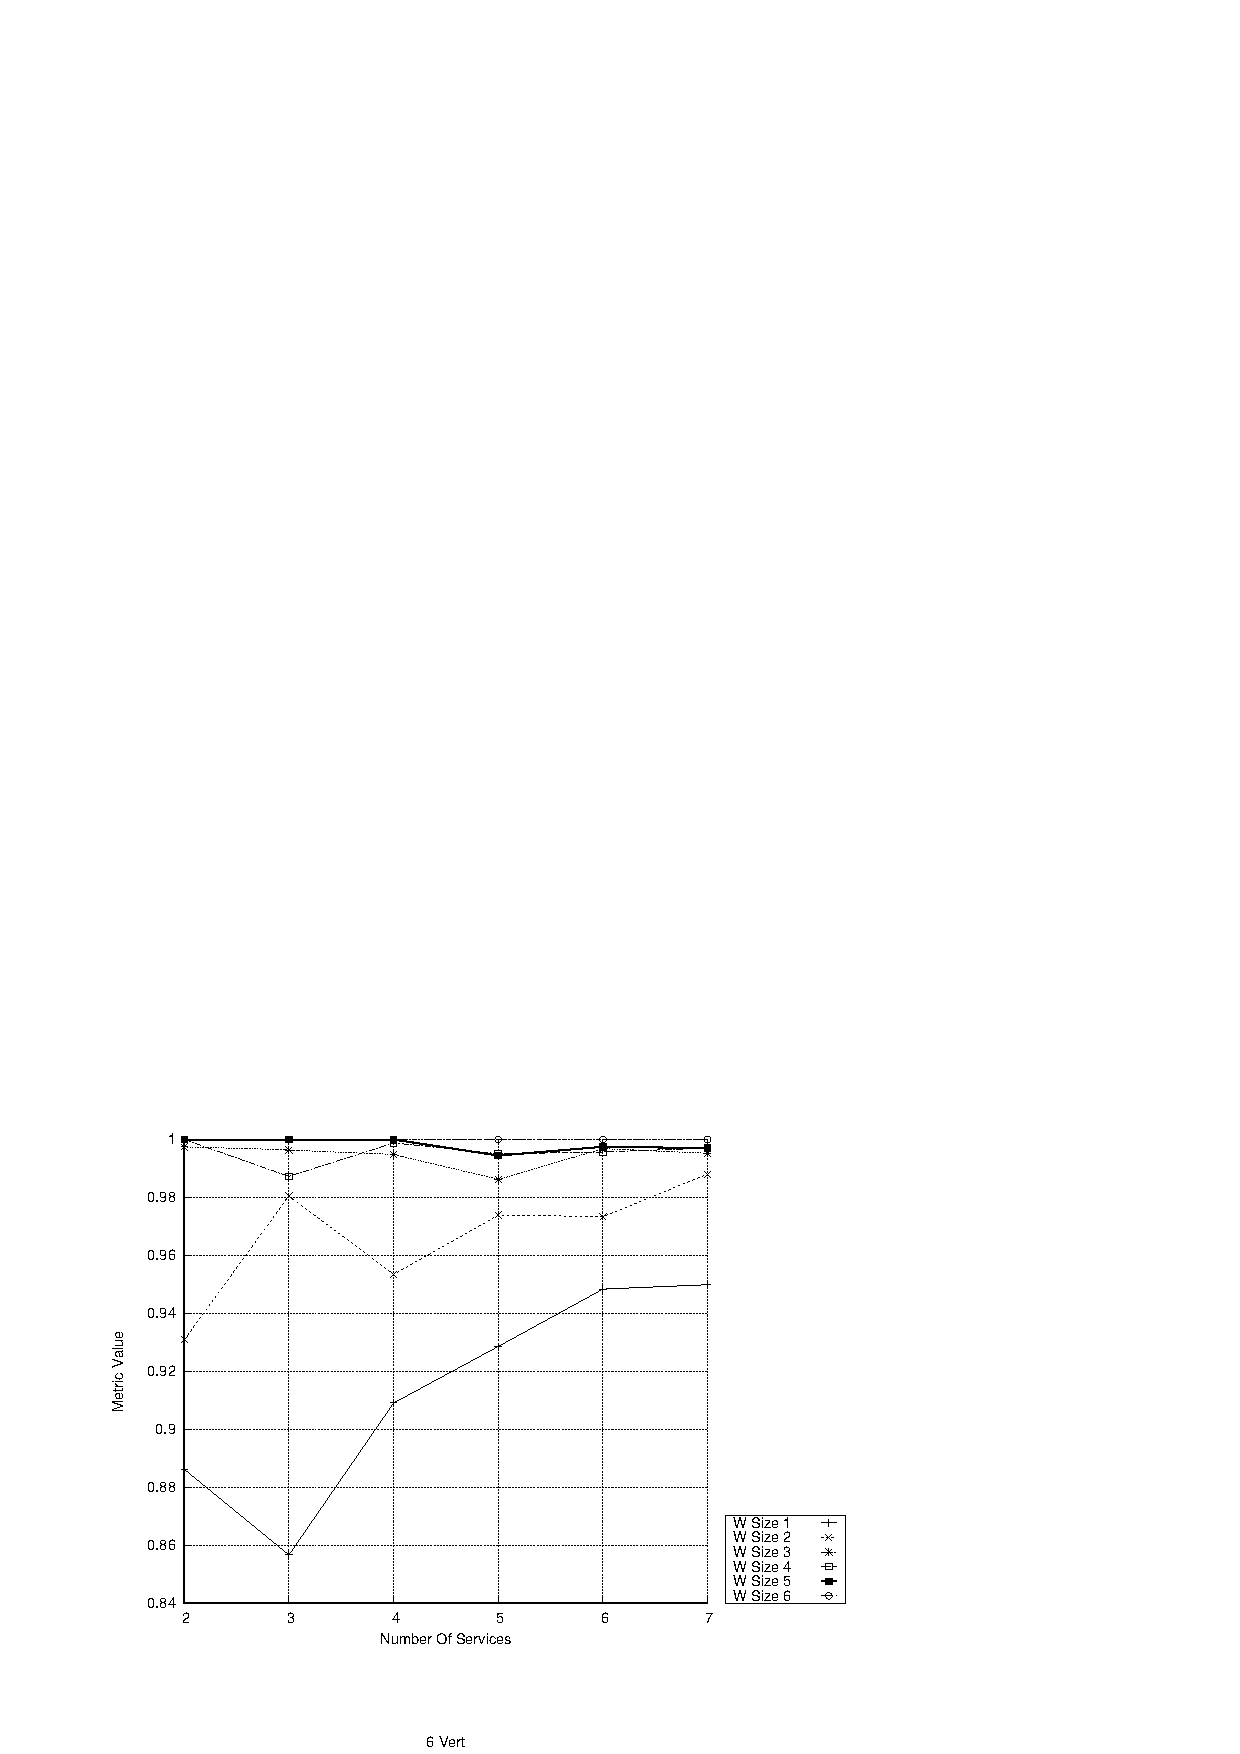
\includegraphics[width=\textwidth]{Images/graphs/window_quality_performance_diff_qual_n7_s7_20_100_n6}
    \caption{6 vertices}
    \label{fig:quality_window_wide_qualitative_n6}
  \end{subfigure}
  \begin{subfigure}{0.33\textwidth}
    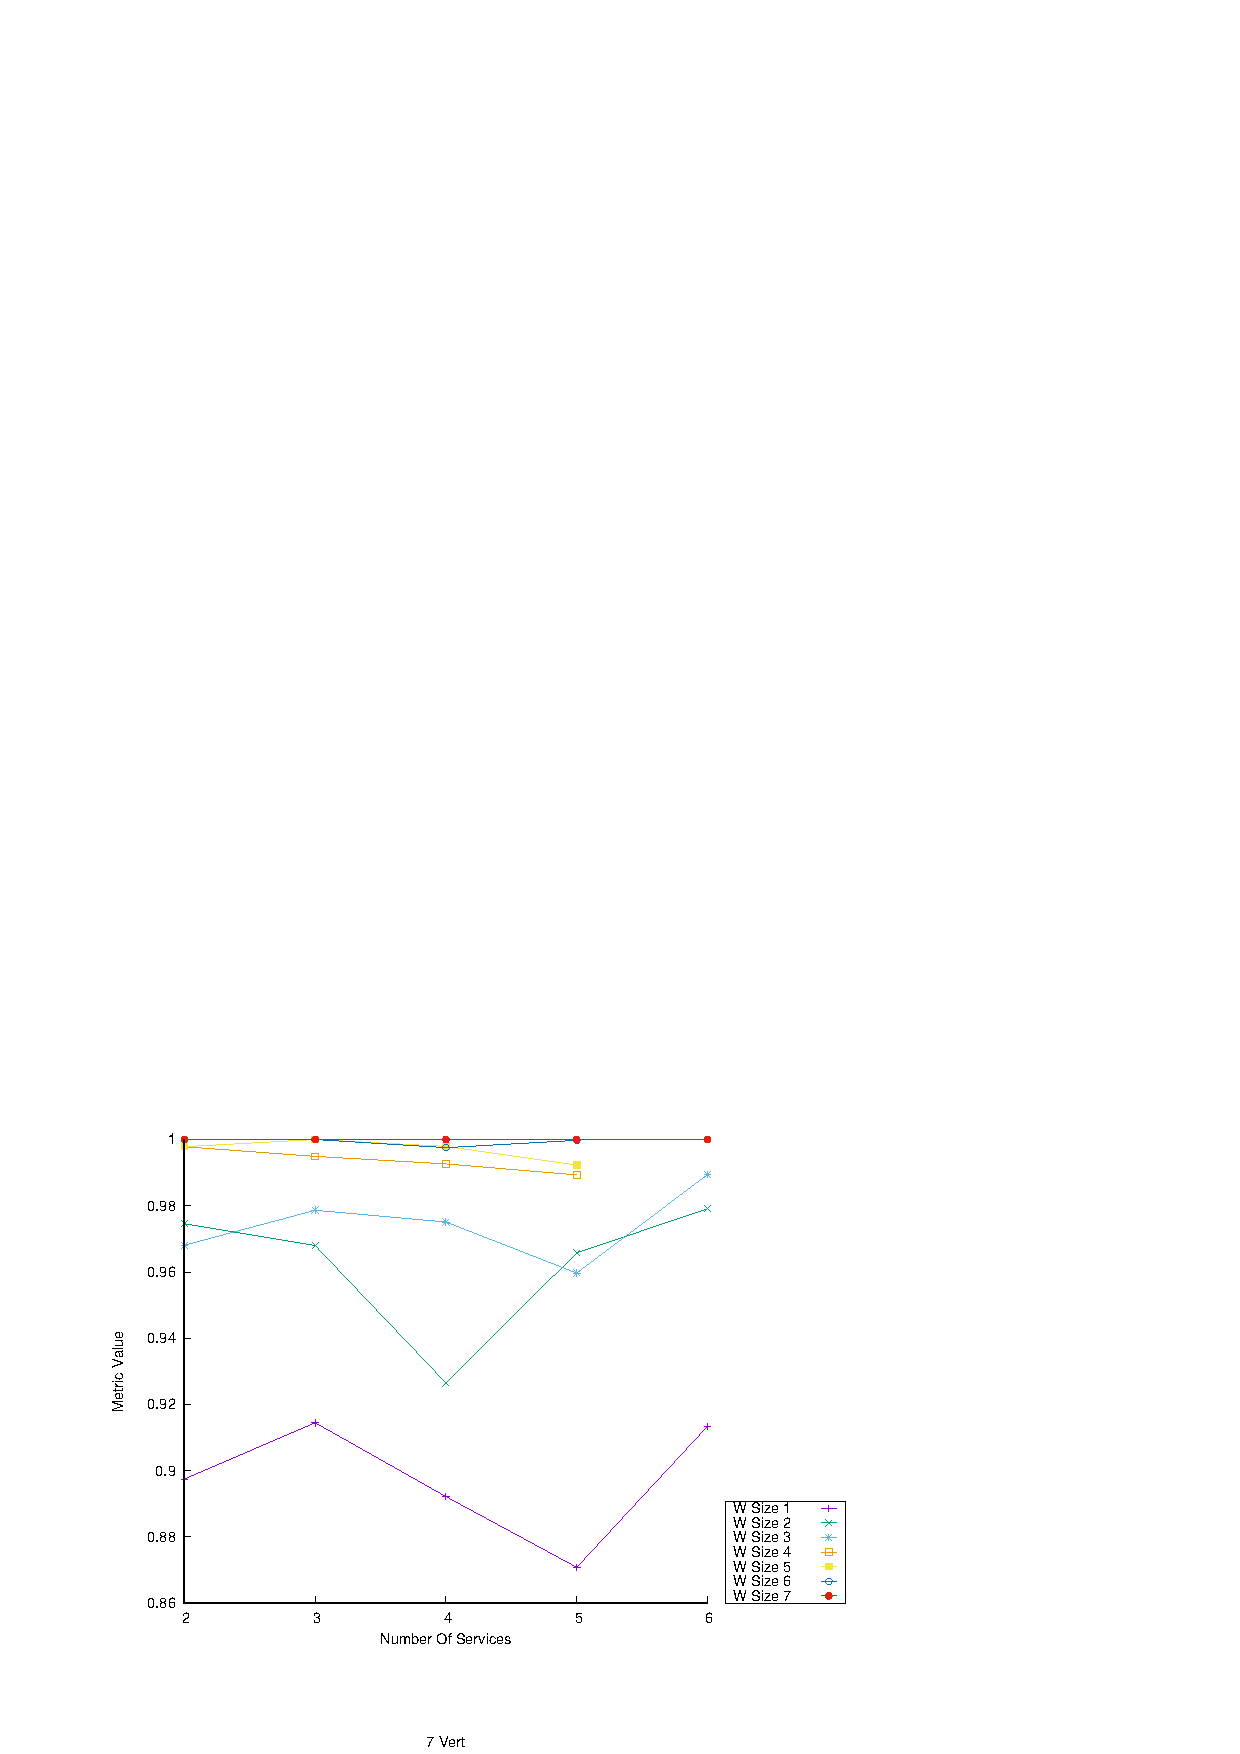
\includegraphics[width=\textwidth]{Images/graphs/window_quality_performance_diff_qual_n7_s7_20_100_n7}
    \caption{7 vertices}
    \label{fig:quality_window_wide_qualitative_n7}
  \end{subfigure}

  \caption{ Quality evaluation with \wide profile.}
  \label{fig:quality_window_wide_qualitative}
\end{figure*}

\begin{figure*}[!htb]
  \centering
  \begin{subfigure}{0.33\textwidth}
    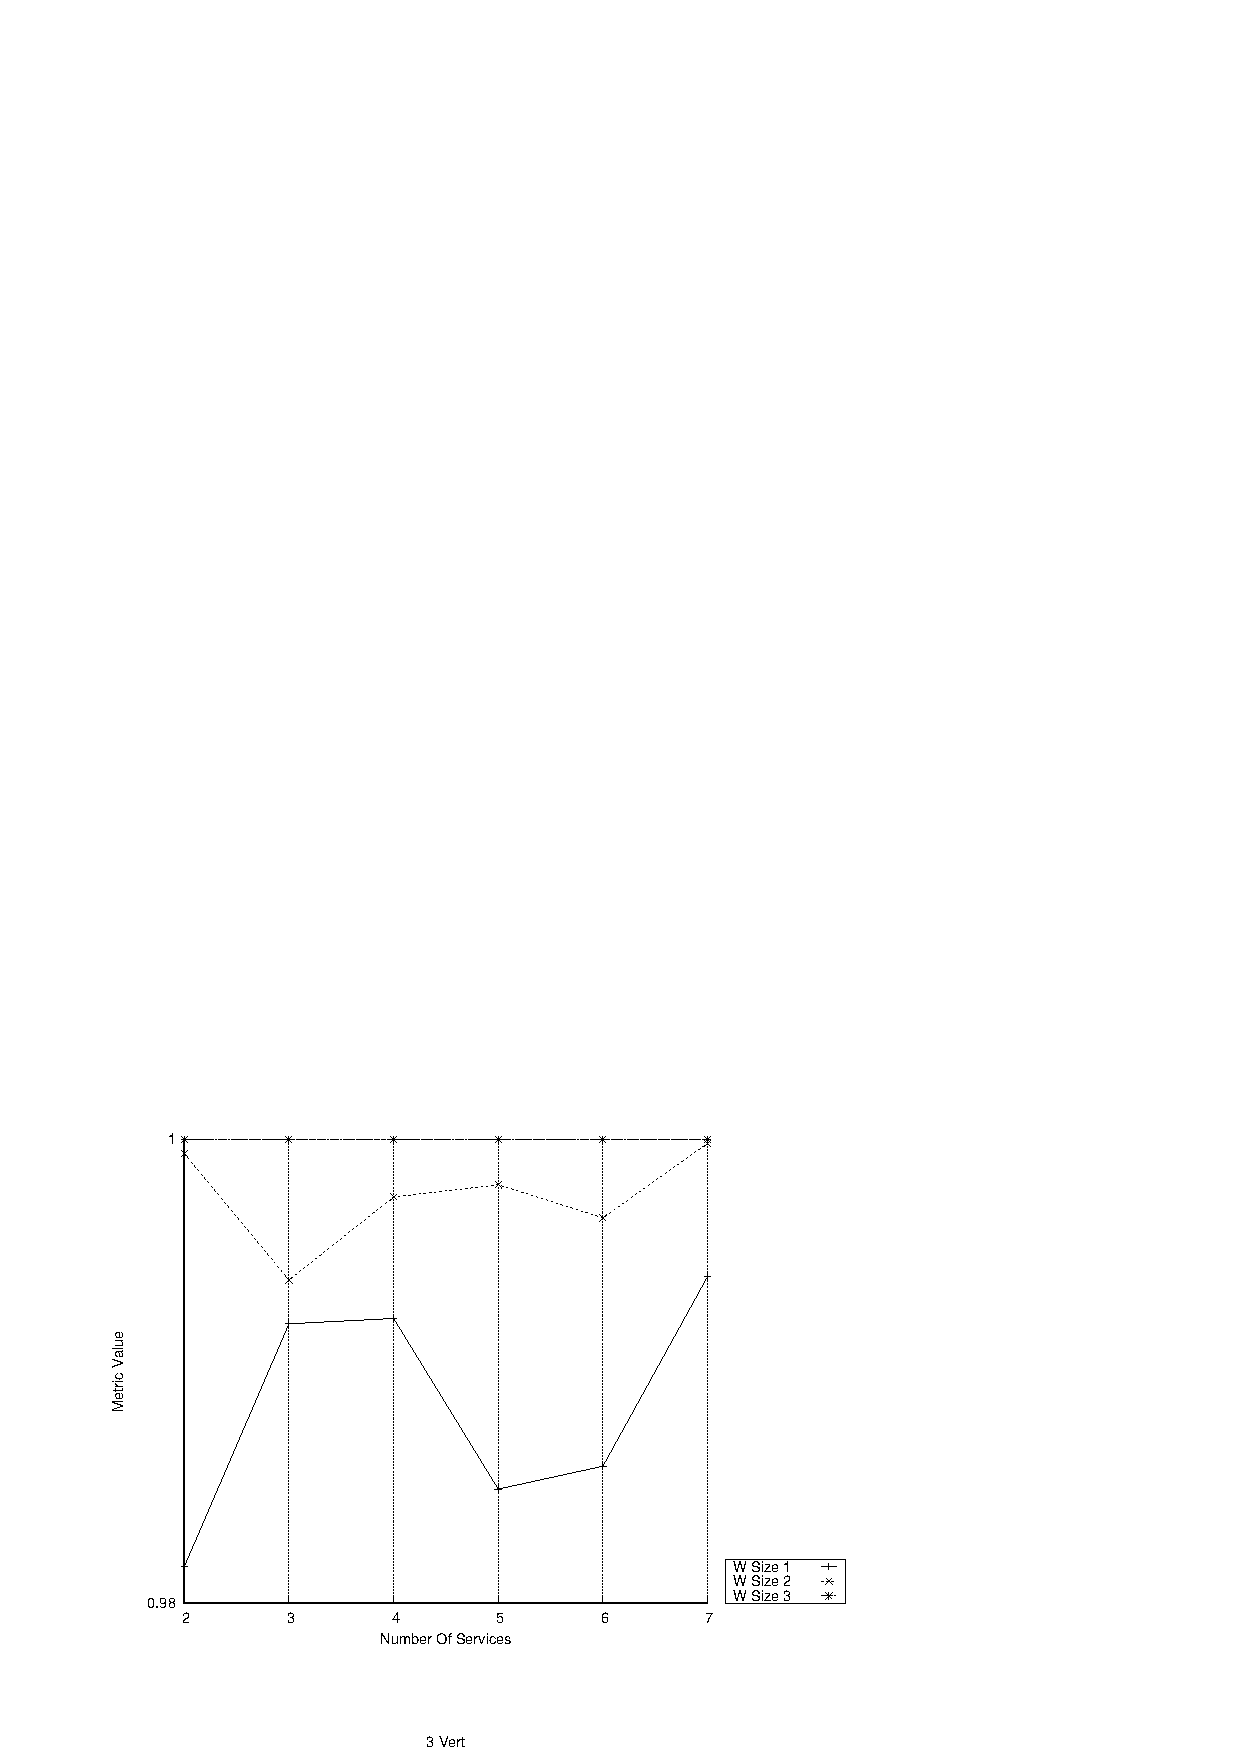
\includegraphics[width=\textwidth]{Images/graphs/window_quality_performance_diff_qual_n7_s7_50_80_n3}
    \caption{3 vertices}
    \label{fig:quality_window_average_qualitative_n3}
  \end{subfigure}
  \hfill
  \begin{subfigure}{0.33\textwidth}
    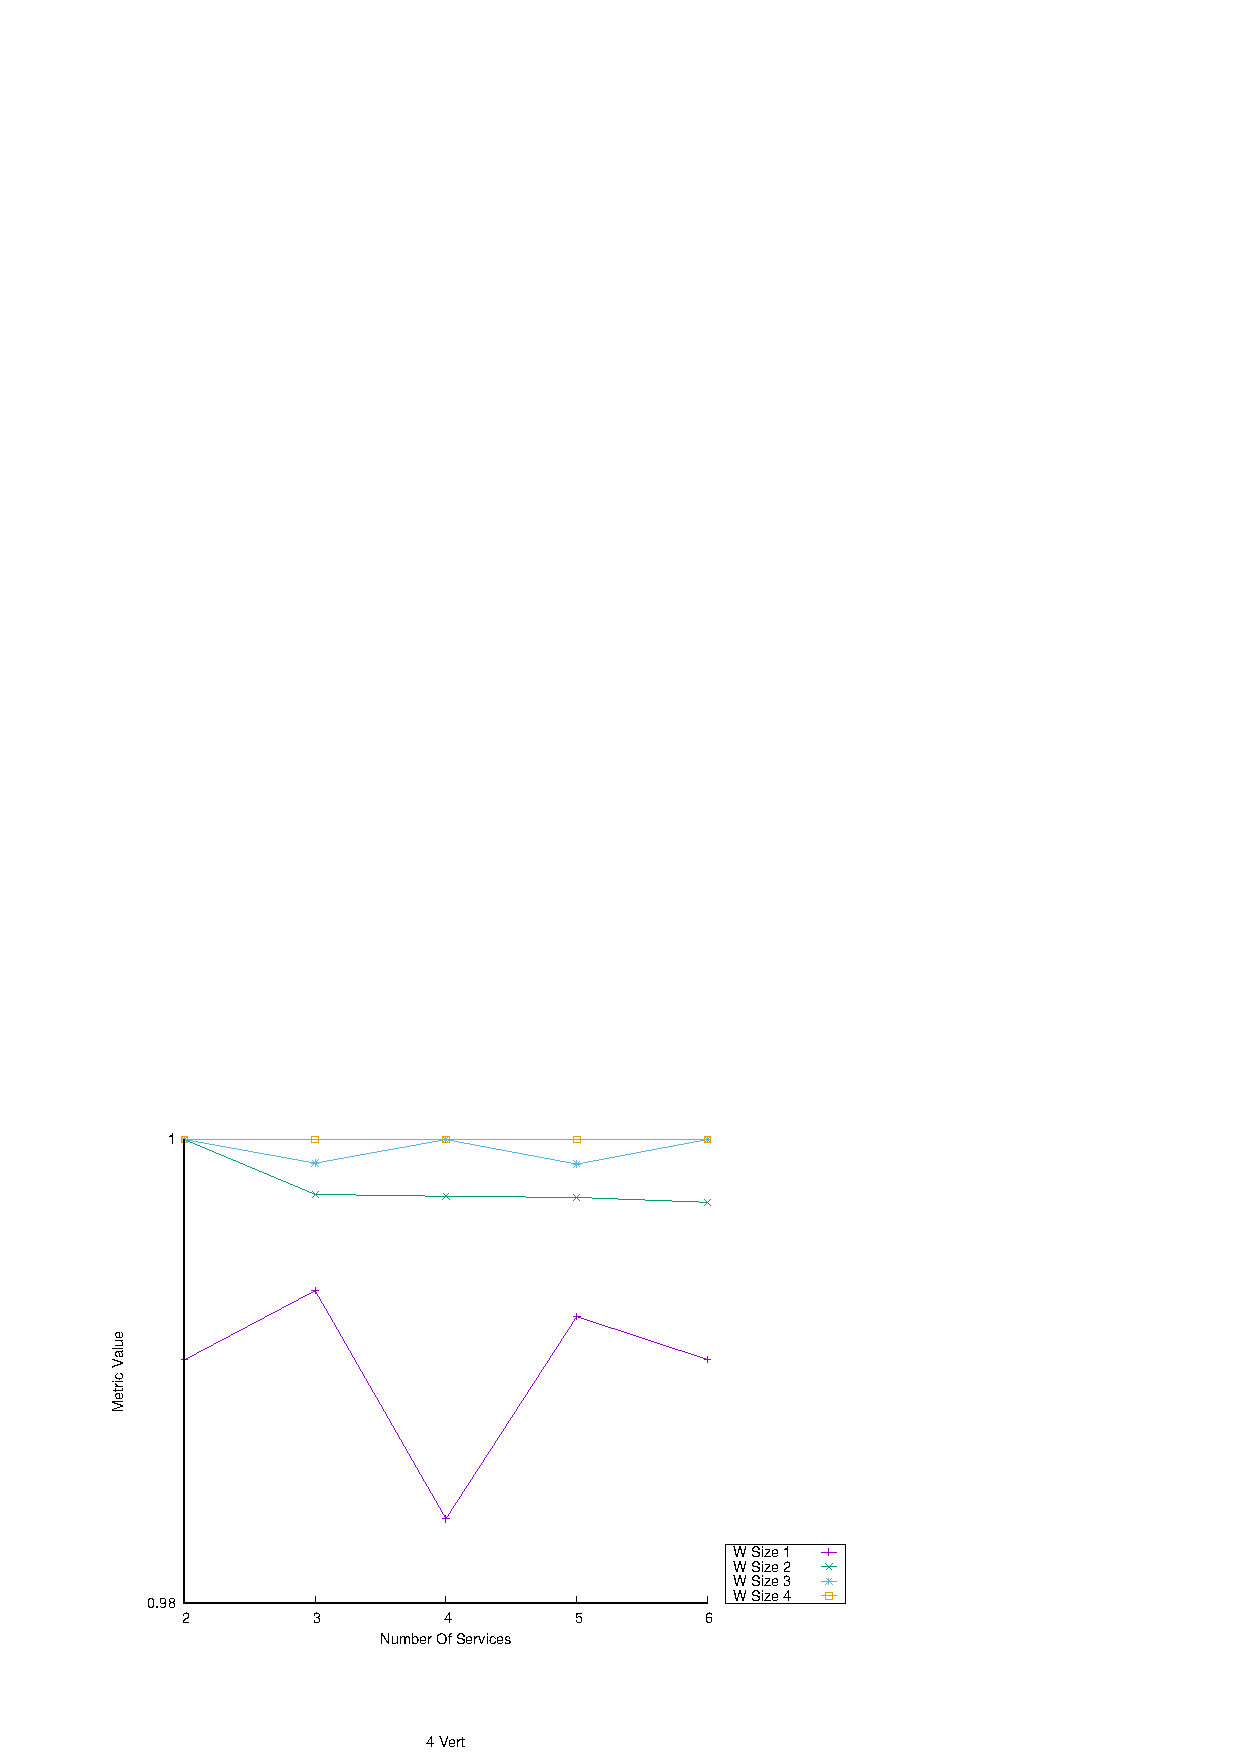
\includegraphics[width=\textwidth]{Images/graphs/window_quality_performance_diff_qual_n7_s7_50_80_n4}
    \caption{4 vertices}
    \label{fig:quality_window_average_qualitative_n4}
  \end{subfigure}
  \hfill
  \begin{subfigure}{0.33\textwidth}
    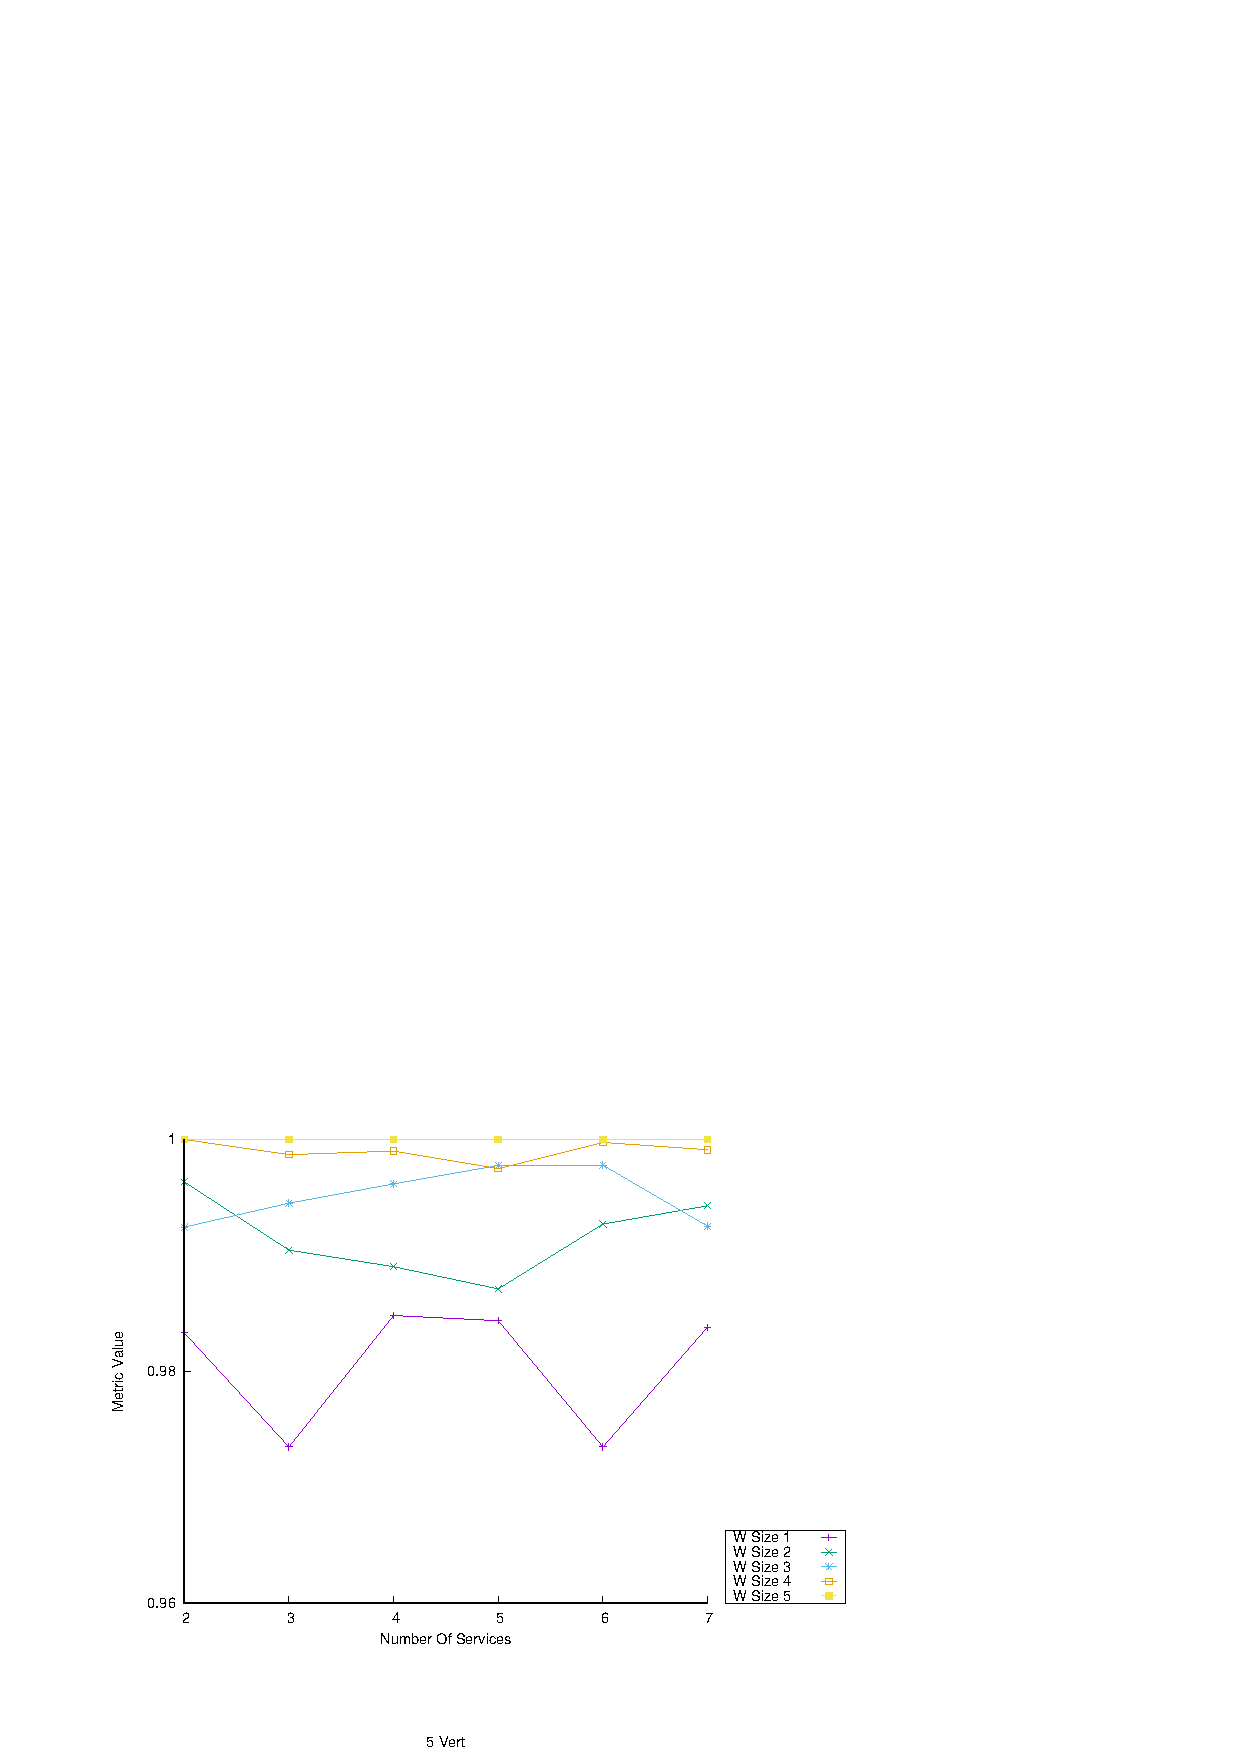
\includegraphics[width=\textwidth]{Images/graphs/window_quality_performance_diff_qual_n7_s7_50_80_n5}
    \caption{5 vertices}
    \label{fig:quality_window_average_qualitative_n5}
  \end{subfigure}
  \hfill
  \begin{subfigure}{0.33\textwidth}
    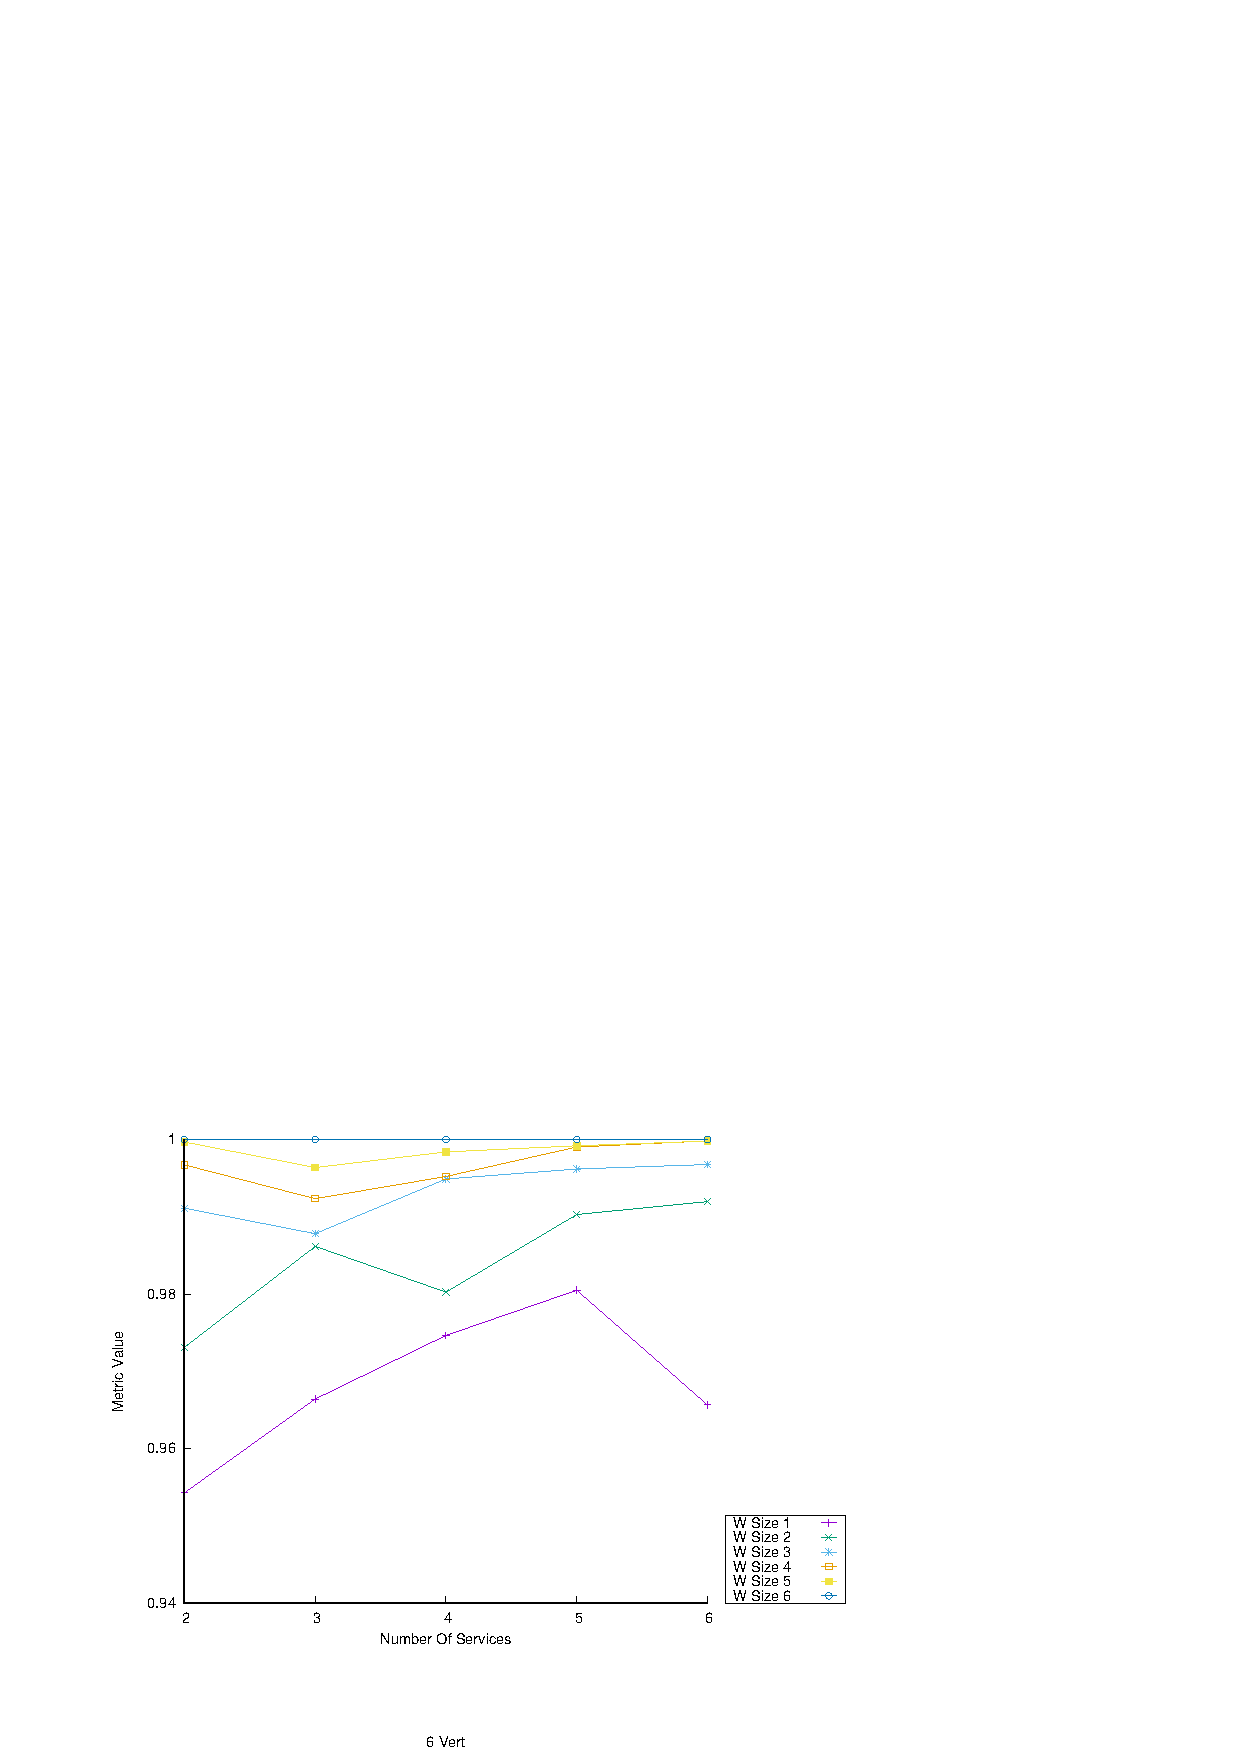
\includegraphics[width=\textwidth]{Images/graphs/window_quality_performance_diff_qual_n7_s7_50_80_n6}
    \caption{6 vertices}
    \label{fig:quality_window_average_qualitative_n6}
  \end{subfigure}
  \begin{subfigure}{0.33\textwidth}
    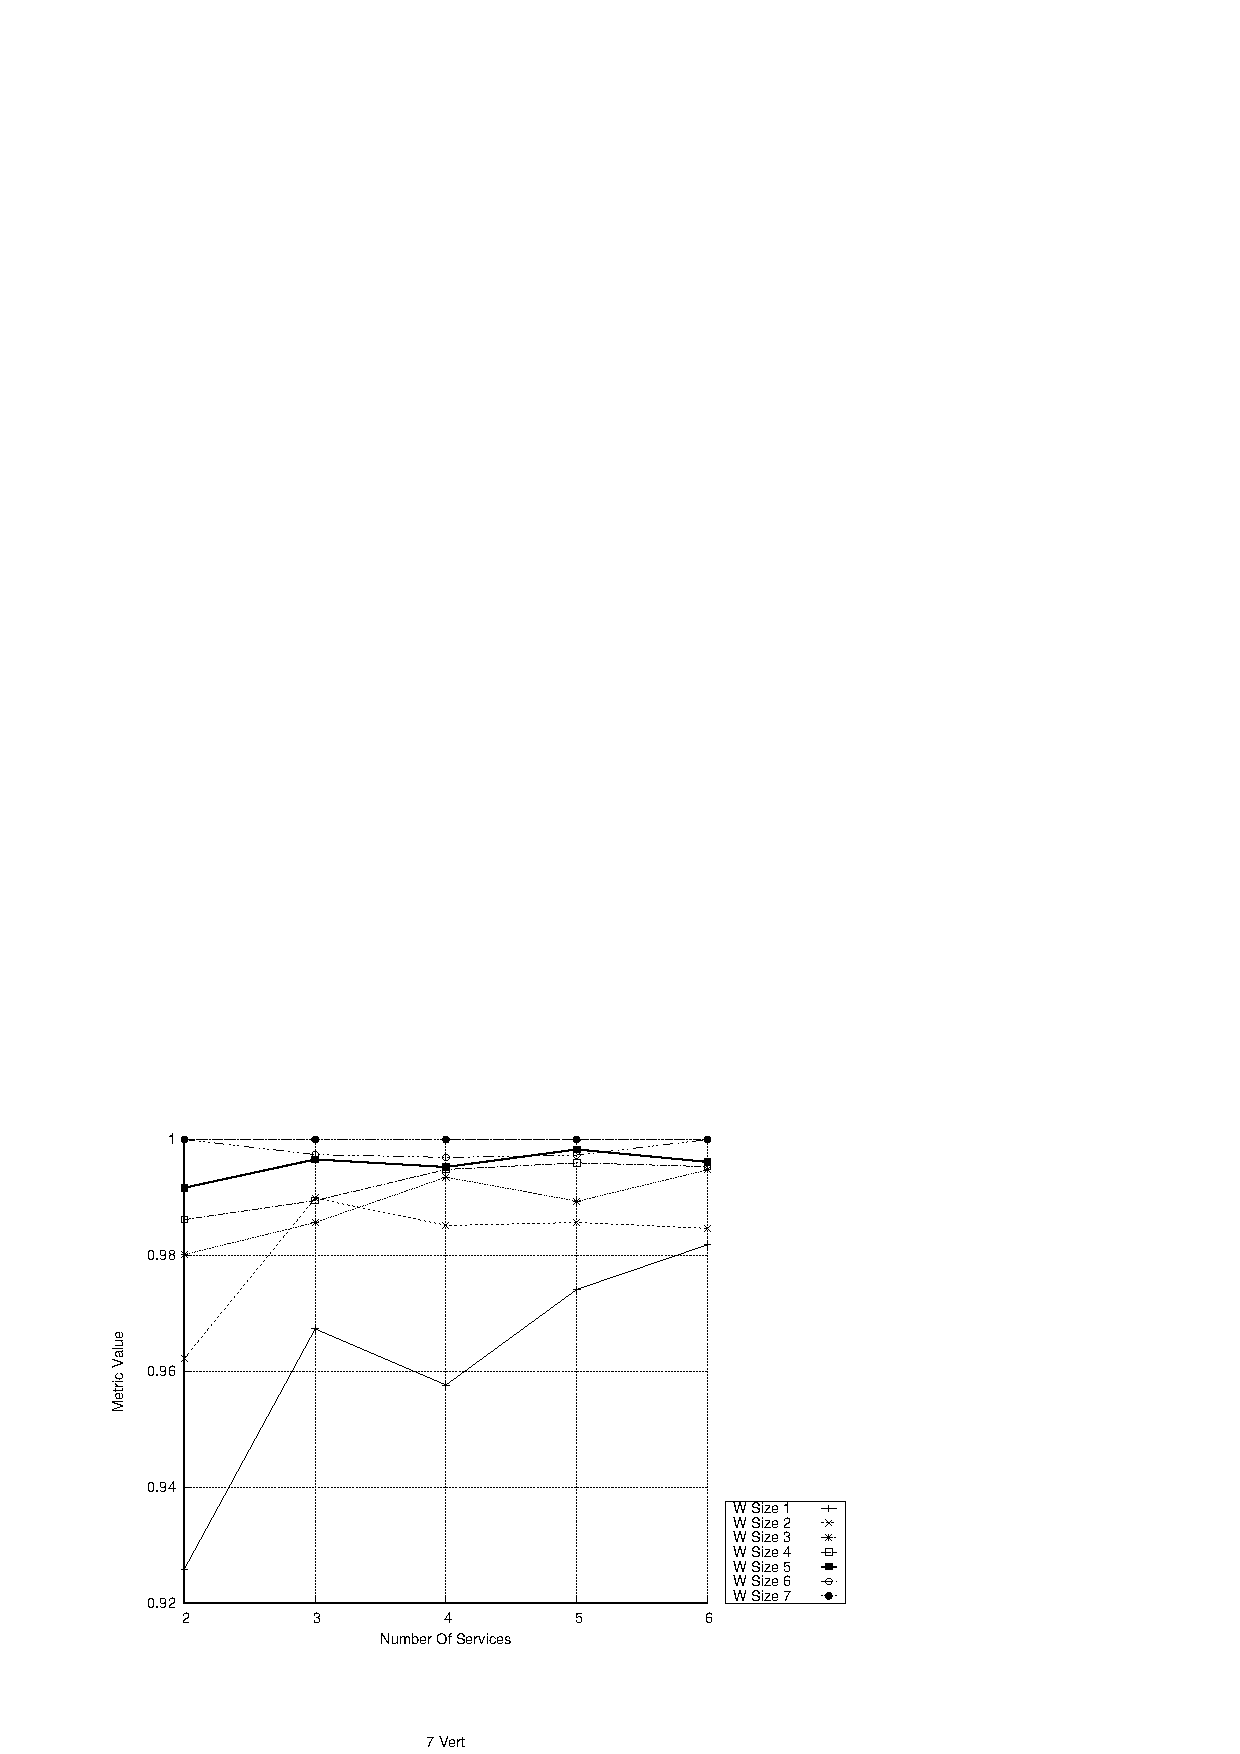
\includegraphics[width=\textwidth]{Images/graphs/window_quality_performance_diff_qual_n7_s7_50_80_n7}
    \caption{7 vertices}
    \label{fig:quality_window_average_qualitative_n7}
  \end{subfigure}

  \caption{ Quality evaluation with \wide profile.}
  \label{fig:quality_window_average_qualitative}
\end{figure*}


